\section{Introduction}

Hopfield Networks were invented by John Hopfield in 1982 under the name of \textit{associative neural network}. They are content addressable binary memory systems that are insensitive to small errors used to model associative memory problems: 
\begin{quote}
\textit{Store a set of $p$ patterns $\psi_i^\mu$ in such a way that when presented with a new pattern $\zeta_i$, the network responds by producing whichever one of the stored patterns most closely resembles $\zeta_i$} \citep{Polk:2002fk}
\end{quote}

\begin{comment}
\begin{wrapfigure}{r}{6cm}
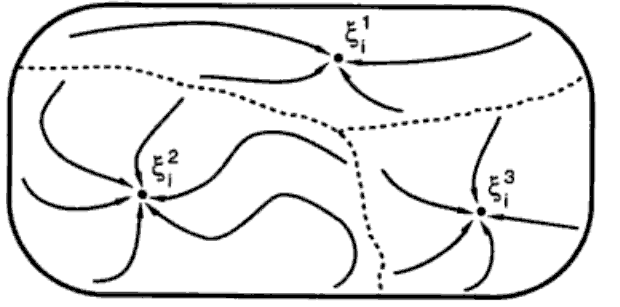
\includegraphics[width=6cm,angle=0]{PatternAttractors.png}
\caption{Configuration space showing the patterns as attractors}
\label{fig:PatternAttractors}
\end{wrapfigure}
\end{comment}



The standard approach to the Hopfield Network includes the use of Hebbian type correlations between pixels. When analyzing one pattern, 


In order to facilitate the mathematical computation, the basis of the binary system is changed from a $\{0,1\}$ base to a $\{-1,1\}$ base, where $-1$ represents a firing neuron. We furthermore denote the pixels by $S_i$ and there correlations by $\omega_{ij}$. The dynamics of the Hopfield Network are then given by:
\begin{equation}
S_i := sign \left( \sum_j \omega_{ij} S_j \right)
\label{eq: sequential dynamics}
\end{equation}
Here $sign$ is defined in an asymmetric way, meaning that $sign(0)=1$. 
When running the dynamics of a Hopfield Network, it can be run synchronously or asynchronously. When run synchronously, the pixels $S_i$ are all updated in the same instance. Asynchronous dynamics allow for the inclusion of data from pixels that have already been changed by running the dynamics on each pixel consecutively. In order to better simulate a biological neuron network, the updating sequence should be random, when running asynchronous dynamics. 

There are many possible exit conditions to the dynamics. The most basic exit condition is probably that the network settles into a stable condition, meaning that no pixels change any more. 

\subsection{The weights}
When analysing just one pattern $\xi_i$, the stable condition becomes very simple and can be given by:
\begin{equation}
sgn\left( \sum_j^N \omega_{ij} \xi_j \right) = \xi_j, \quad	\forall i
\end{equation}
This is clearly the case for all $\omega_{ij}=\frac{1}{N} \xi_i \xi_j$. This formalism clearly retains the insensitivity of the Hopfield Network to minor errors in the pattern, since even if some pixels are wrong, as long as it is less then half the pixels, equation \ref{eq: sequential dynamics} will still give the correct result and produce $\xi_i$. $\xi_i$ is therefore called an \textbf{attractor}. For each attractor there must be a second attractor called the \textbf{reversed state} $-\sigma$, which is reached when more than half of the pixels are faulty. 
When trying to recall the most similar pattern out of several patterns, we can define the weights as a superposition of the individual weights for $p$ patterns:
\begin{equation}
\omega_{ij}=\frac{1}{N} \sum_{mu=1}^p \xi_i^\mu \xi_j^\mu
\end{equation}

